\clearpage
\section{Reduksjon av modeller med time scale og kapasitet}\label{sec:timescale}
En modell er alltid bygget på et sett med antagelser som divergerer modellen fra det reelle. Frem til nå har vi gjort antagelser på kapasitet og time scale uten å være fullt klar over argumentene for antagelsene. Time scale assumptions er kort fortalt neglisjering av modeller pga dynamiske forskjeller. Vi kan dele en time scale inn i tre deler:


\begin{itemize}
    \item Event dynamic: Skjer  umiddelbart
    \item Dynamisk: Forandring over tid som er merkbart
    \item Konstant: Ingen forandring i system
\end{itemize}

\begin{figure}[H]
    \centering
    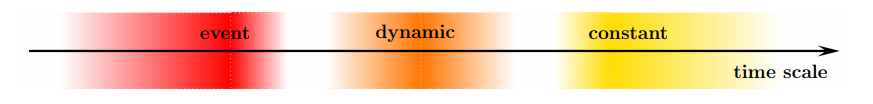
\includegraphics[scale=0.5]{Figures/time_scale}
    \caption{Time scale som visualiserer hvordan event, dynamic og constant henger sammen. Merk at ingen av domenene overlapper.}
    \label{fig:time_scale}
\end{figure}


Vi har mange måter å gå fram på for å redusere modeller. Vi bruker i hovedsak 4 angrepsvinkler. De fire forskjellige metodene blir nærmere forklart i det kommende eksempelet i \cref{sec:tre_sjo}. 
\begin{enumerate}
    \label{lst:reduction}
    \item Ekspandere det som er konstant
    \item Introdusere event dynamic
    \item Analysere den raske dynamikken
    \item Analysere den trege dynamikken
\end{enumerate}

\subsection{Eksempel: Tre innsjøer}\label{sec:tre_sjo}
Vi ønsker å modellere vannet som renner fra en stor innsjø (R) til en mindre (C) og videre til en enda mindre innsjø (S). For å forklare reduksjonen best mulig trekker vi fram en enkel topologi:


\begin{figure}[H]
    \centering
    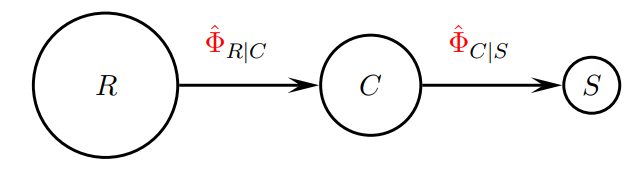
\includegraphics[scale=0.5]{Figures/time_scale_topo}
    \caption{Topologi for tre innsjøer hvor R transporterer til C som transporterer til S.}
    \label{fig:time_scale_topo}
\end{figure}

Den fulle modellen for topologien for \cref{fig:time_scale_topo} gir likningene:
\begin{align}
    \dot{\Phi}_{R} =&\, -\hat{\Phi}_{R|C} \\
    \dot{\Phi}_C =&\, \hat{\Phi}_{R|C} - \hat{\Phi}_{C|S}\\
    \dot{\Phi}_S =&\, \hat{\Phi}_{C|S}
\end{align}

Vi gjør reduksjon ved bruk av de fire angrepsvinklene. I ABC-heftet kapittel 16 har de en matematisk forklaring på reduksjonen, den har vi valgt å ikke ta med til fordel for den intuitive forklaringen.  

\begin{center}
    \textbf{1:} Ekspandere det som er konstant.
\end{center}
Ved å anta at R er mye større enn C og S så kan vi observere R som et reservoar som fører til at vi ikke trenger å modellere R ($\underline{\dot{\Phi}}_R = 0$).

\begin{figure}[H]
    \centering
    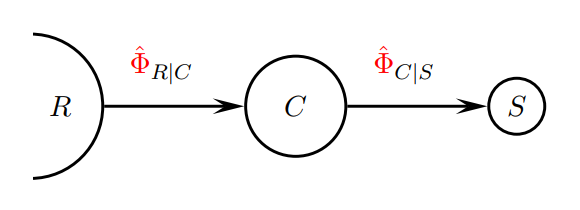
\includegraphics[scale=0.5]{Figures/time_scale_topo1.png}
    \caption{Topologi for tre innsjøer hvor R er betydelig mye større enn C og S.}
    \label{fig:time_scale_topo1}
\end{figure}
Dette gir oss en ny modell:
\begin{align}
    \dot{\Phi}_C =&\, \hat{\Phi}_{R|C} - \hat{\Phi}_{C|S}\\
    \dot{\Phi}_S =&\, \hat{\Phi}_{C|S}
\end{align}


\begin{center}
    \textbf{2:} Introdusere event dynamic.
\end{center}

Hvis vi antar at volumet S er minimalt forhold til C, kan vi anta at det som går ut av C til S er neglisjerbart forhold til transporten fra R til C.

\begin{figure}[H]
    \centering
    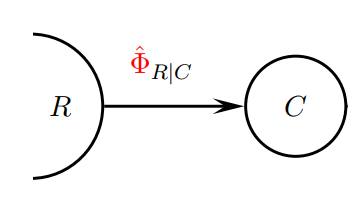
\includegraphics[scale=0.5]{Figures/time_scale_topo2.png}
    \caption{Topologi for tre innsjøer hvor transporten fra C til S er så minimal at det ikke har noen påvirkning på modellen.}
    \label{fig:time_scale_topo2}
\end{figure}



\begin{center}
    \textbf{3:} Analysere den raske dynamikken (small time scale).
\end{center}

Vi tar fram topologien i \cref{fig:time_scale_topo1}, etter ekspansjonen av det konstante domenet, og setter inn en lineær modell for transport som vi lærte i \cref{sec:linear_transport}.

\begin{align}
    \dot{\Phi}_C =&\, \hat{\Phi}_{R|C} - \hat{\Phi}_{C|S}\\
    \dot{\Phi}_S =&\, \hat{\Phi}_{C|S} \\[0.5cm]
    \dot{\Phi}_C =&\, -k_{R|C}(\pi_C-\pi_R) +k_{C|S}(\pi_S-\pi_C)\\
      \dot{\Phi}_S =&\ -k_{C|S}(\pi_S-\pi_C)
\end{align}

Ved å anta at transporten $\hat{\Phi}_{R|C}$ er mye tregere enn  $\hat{\Phi}_{C|S}$ kan vi anta at ved en liten time scale vil $\hat{\Phi}_{C|S}$ dominere og vi kan neglisjere transporten fra R til C i $\dot{\Phi}_C$:

\begin{align}
    \dot{\Phi}_C =&\, +k_{C|S}(\pi_S-\pi_C)\\
      \dot{\Phi}_S =&\ -k_{C|S}(\pi_S-\pi_C)
\end{align}

\begin{center}
    \textbf{4:} Analysere den trege dynamikken (large time scale).
\end{center}

Å bruke en lang time scale er veldig vanlig i prosessmodellering. Etter en lang tid vil forskjellen i effort variabler, mellom de to systemene, forsvinne. Tenk deg at du har laget deg en kopp med varm kaffe. Venter du i 24 timer før du drikker kaffen kan du forvente at temperaturen til koppen er den samme som rommet. 

\begin{align}
    0 =&\, k(\pi_S - \pi_C) \\
    \pi_C =&\, \pi_S
\end{align}